\documentclass[11pt]{article}
\usepackage[utf8]{inputenc}
\usepackage{amsfonts}
\usepackage{natbib}
\usepackage{graphicx}
\usepackage{amsmath}
\usepackage{amssymb}
\usepackage{mathrsfs} % Cursive font
\usepackage{graphicx}
\usepackage{ragged2e}
\usepackage{fancyhdr}
\usepackage{nameref}
\usepackage{wrapfig}
\usepackage{listings}

% to set spacing between lines
\usepackage{setspace}

% to rotate content 90 degrees
\usepackage{lscape}



% defining command for the curly arrow
\newcommand{\curly}{\mathrel{\leadsto}}


\usepackage{mathtools}
\usepackage{xparse} \DeclarePairedDelimiterX{\Iintv}[1]{\llbracket}{\rrbracket}{\iintvargs{#1}}
\NewDocumentCommand{\iintvargs}{>{\SplitArgument{1}{,}}m}
{\iintvargsaux#1}
\NewDocumentCommand{\iintvargsaux}{mm} {#1\mkern1.5mu,\mkern1.5mu#2}

\makeatletter
\newcommand*{\currentname}{\@currentlabelname}
\makeatother

\usepackage[a4paper,hmargin=1in, vmargin=1.4in,footskip=0.25in]{geometry}


%\addtolength{\hoffset}{-1cm}
%\addtolength{\hoffset}{-2.5cm}
%\addtolength{\voffset}{-2.5cm}
\addtolength{\textwidth}{0.2cm}
%\addtolength{\textheight}{2cm}
\setlength{\parskip}{8pt}
\setlength{\parindent}{0.5cm}
\linespread{1.5}

\pagestyle{fancy}
\fancyhf{}
\rhead{TP1 - Sullivan}
\lhead{Seguridad Informática}
\rfoot{\vspace{1cm} \thepage}

\renewcommand*\contentsname{\LARGE Índice}

\begin{document}

\begin{titlepage}
    \begin{center}
        \vfill
        \vfill
            \vspace{0.7cm}
            \noindent\textbf{\Huge Trabajo Práctico 1}\par
            \noindent\textbf{\Huge Seguridad Informática}\par
            \vspace{.5cm}
        \vfill
        \noindent \textbf{\huge Alumna:}\par
        \vspace{.5cm}
        \noindent \textbf{\Large Sullivan, Katherine}\par
 
        \vfill
        \large Universidad Nacional de Rosario \par
        \noindent\large 2023
    \end{center}
\end{titlepage}
\ \par


% Setting the spacing between lines
\setstretch{0}

\section*{Selección de ejercicios en el conjunto \{2,3,4\} - Ejercicio 3}

\textbf{Discuta cómo las políticas de seguridad y los modelos para hacerlas cumplir pueden imponer
barreras comerciales}

Existen distintas maneras en las que las políticas de seguridad y los modelos para hacerlas cumplir pueden imponer barreras comerciales. 

En primera instancia, se podría pensar en los \textbf{costos} que se derivan al intentar crear y cumplir con políticas de seguridad rigurosas, pues las organizaciones deben invertir en tecnología, capacitación y personal especializado. 

En segundo lugar, se podría pensar en la \textbf{baja de productividad} (que también lo podríamos pensar como un costo en tiempo) al, por restricciones de seguridad, no poder hacer uso de herramientas tecnológicas que realizarían alguna tarea de manera rápida y efectiva, o al \textbf{limitar la colaboración y la flexibilidad} entre miembros de un equipo por restricciones en cuanto al acceso de la información y los distintos sistemas.

En tercer lugar, se podría pensar en los \textbf{costos burocráticos} de procesos que sin políticas de seguridad podrían ser más fácil como la descarga de aplicaciones, el agregado de usuarios, etc. 

Y, por último lugar, se podría pensar en el posible \textbf{impacto negativo en la experiencia del usuario}. Medidas de seguridad un producto o servicio tecnológico podrían generarle molestias a un usuario final, quien podría decidir no usar más el producto o servicio por esta razón, lo cual es una gran pérdida.

Todas estas descentajas podrían llevar a pensar que no es tan buena idea tener políticas de seguridad, sin embargo, hay que aclarar y nos debemos llevar la idea de que cualquier tipo de costo preventivo que se tenga respecto a políticas de seguridad es ampliamente inferior a lo costoso que resulta el tener un grave problema de seguridad.

\section*{Selección de ejercicios en el conjunto \{7,8,9\} - Ejercicio 9}

\textbf{El aforismo “seguridad a través de oscuridad” sugiere que el ocultamiento de información provee
algún grado de seguridad. Dé un ejemplo de alguna situación en que el ocultamiento de información
no agrega apreciable seguridad a un sistema. Luego dé un ejemplo en que sí.}

Se podría pensar que una situación donde el ocultamiento de información no provee seguridad es el ocultamiento de contraseñas débiles. Si bien las contraseñas débiles no serían encontradas, al ser fácilmente adivinables la medida de seguridad se rompe fácilmente.

Un ejemplo donde el ocultamiento si provee buena seguridad es, por ejemplo, usar puertos personalizados, manteniendo cuáles bien ocultos, para evitar ataques que se hacen a los puertos conocidos. Mientras a la vez se mantengan los apropiados firewalls y medidas de seguridad pertinentes en este caso la ocultación está proveyendo una mayor seguridad. 

\section*{Selección de ejercicios en el conjunto \{13, 14, 15\} - Ejercicio 13}

\textbf{Lea sobre el modelo de Biba para integridad}

El modelo Biba es un modelo de seguridad que se utiliza para garantizar la integridad de los datos en un sistema de información. 

Este modelo se caracteriza por la frase: ``leer hacia arriba, escribir hacia abajo". Esto contrasta con el modelo Bell-LaPadula, que se caracteriza por la frase ``leer hacia abajo, escribir hacia arriba".

En el modelo Biba, los usuarios solo pueden crear contenido en o por debajo de su propio nivel de integridad, mientras que los usuarios solo pueden ver contenido en o por encima de su propio nivel de integridad, llevando nombres estas propiedades:

Propiedad de Integridad Simple: establece que un sujeto en un nivel de integridad dado no debe leer datos en un nivel de integridad inferior (no leer hacia abajo).

Propiedad de Integridad * (estrella): establece que un sujeto en un nivel de integridad dado no debe escribir en datos en un nivel de integridad superior (no escribir hacia arriba).

Además, la Propiedad de Invocación establece que un proceso de un nivel inferior no puede solicitar un acceso superior; solo puede hacerlo con sujetos que estén en un nivel igual o inferior.

Todo esto nos lleva a darnos cuenta que este modelo toma el enfoque opuesto al modelo Bell-LaPadula.

\textbf{¿Es posible usar los modelos de Bell-LaPadula y de Biba para modelar confidencialidad e
integridad simultáneamente? ¿Se pueden usar las mismas categorĺas de seguridad para ambas
políticas}

Resulta posible usarlos en simultáneo. 

En el caso de tener clases opuestas para integridad y confidencialidad, los modelos simplemente abogarían por lo mismo y sería lo mismo tener ambos o uno solo. 

En el caso de tener clases iguales, un usuario solo podría acceder a los objetos clasificados con su mismo nivel, lo que lo haría muy restrictivo. 

En general, entiendo que, en caso de combinarlos, se buscaría utilizar categorías distintas para abordar estos problemas de manera particular.

\section*{Inciso a elección del ejercicio 21 - Programa 2}

\textbf{Determine si hay flujo indebido de información en este programa}

\begin{lstlisting}
    x = readH();
    writeL("Loading...");
    writeH(x);
\end{lstlisting}

Si bien podemos observar que hay una lectura de un archivo clasificado como high y una escritura en un archivo clasificado con low, 
como esta escritura no se encuentra de ninguna manera condicionada por la lectura y se descarta la posibilidad de un filtrado de información 
por un timing channel, se determina que en el programa no hay un flujo indebido de la información.


\section*{Inciso a elección del ejercicio 22 - Programa 2}
\textbf{Para el programa del ejercicio anterior, explique cómo funcionaría la ejecución bajo el
sistema de seguridad por multi-ejecución}

\begin{lstlisting}
    x = readH();
    writeL("Loading...");
    writeH(x);
\end{lstlisting}

En SME en principio el pograma se lanzaría clasificado como low. 

Al momento de realizar la lectura del archivo clasificado como high (y su posterior asignación a la variable x) se haría un fork, creando dos procesos $P_L$ y $P_H$.
$P_L$ sería el mismo proceso que ejecutaba a nivel L y no se le permitiría acceder a la informaci´on de H mientras que $P_H$ sería un
nuevo proceso clasificado con H al que se le permite acceder a la informaci´on H. 

La instrucción de escritura en el archivo low solo la realizaría el proceso $P_L$, puesto que un proceso clasificado con H solo puede escribir informaci´on en objetos clasificados con H. 

La instrucción de escritura en H, en teoría, la podrían realizar tanto $P_L$ como $P_H$, el problema surge en que si bien $P_H$ tiene acceso a la variable x y la podría escribir tranquilamente, el proceso $P_L$ no.
Qué ejecutaría $P_L$ al encontrarse con esa instrucción dependerá de la implementación específica de SME, en principio, se podría pensar que a x se le asigna un valor predeterminado (como ser 0) y simplemente se escribiría eso, pero 
podría variar.


\section*{Desafío a elección del ejercicio 23 - Desafío 6}

\begin{lstlisting}
    declare proc p(in x : high, out y : high) {
        y = x;
    }
    p(h,l);
\end{lstlisting}

\textbf{¿Qué tipo de ataque logró llevar adelante?}

Se da un ataque de filtrado de información explícito, al asignarle a una varible low (l) explícitamente el valor de una variable high (h) cuando se llama al proceso p.

\textbf{¿Qué limitación tiene el sistema de reglas?}

El sistema de reglas no verifica que las variables pasadas como parámetros realmente estén clasificadas de la manera en las que se las enuncian en el proceso, por eso puede 
realizarse la asignación de una variable high a una variable low (pues el proceso la entiende como high).

\textbf{¿Qué cambio habría que hacerle para impedir el ataque?}

Considero que el cambio más simple para hacer sería modificar la regla presentada para la llamada de procesos

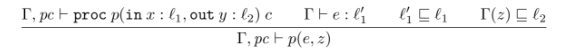
\includegraphics[scale=0.75]{Captura de pantalla de 2023-09-29 20-31-13.png}

de manera tal que verifique que la clasificación de las variables con las que se llama a un proceso coincidan exactamente con aquellas categorías que el proceso le da (no que ``estén contenidas en / sean menores que").

Sin embargo, existen otros posibles cambios, como por ejemplo, no tomar categorizaciones locales de variables en los procesos.

\end{document}
